
\documentclass[a4paper,11pt]{article}

\usepackage{fontspec}
\setmainfont{Calibri}

\linespread{1}

\setlength{\oddsidemargin}{0cm}
\setlength{\evensidemargin}{0cm}
\setlength{\textheight}{23cm}
\setlength{\textwidth}{16cm}

\usepackage{amssymb,mathrsfs,algorithmic,algorithm,multirow}
\usepackage{amsmath,amsbsy,graphicx,color,url,natbib}
\usepackage{ccaption}
\setlength{\bibsep}{0.0pt}

\newcommand{\bm}{\mathbf}
\newcommand{\bs}{\boldsymbol}
\newcommand{\mt}{\mathrm}
\newcommand{\nind}{\noindent}

\usepackage{fancyhdr}
\newcommand{\tstamp}{\today}   
\lhead[\fancyplain{}{\rightmark}]       {\fancyplain{}{}}
\rhead[\fancyplain{}{\rightmark}]       {\fancyplain{}{}}
\chead[\fancyplain{}{\centermark}]       {\fancyplain{}{ENGM214 -- Process Modelling and Simulation} }
\pagestyle{fancyplain}

\usepackage{amsthm}
\theoremstyle{definition}
\newtheorem{exmp}{Example}[section]

\title{\vspace{-2cm} Lecture 6 -- Distributed parameter systems: models and solutions}

\author{Tao Chen\\
{\small \emph{Department of Chemical \& Process Engineering, University of Surrey, UK}}\\
{\small (email: \texttt{t.chen@surrey.ac.uk}; \hspace{0.5cm} updated on \today )}
}
\date{}

\begin{document}
\maketitle

%\tableofcontents
\vspace{-0.5cm}

\section{Modelling distributed parameter systems}

In Lecture 3, we discussed the equation of conservation in both integral and derivation forms.
In this lecture, we will apply these principles and equations to the so-called distributed parameter
systems, that is the extensive variables (mass, energy, momentum) change with spatial position.

We begin by re-writing the general differential form of the conservation equation
in Lecture 3:
\begin{equation} \label{eq:conserv_pds_1}
	\frac{\partial \hat{\Phi}}{\partial t} = - \nabla \cdot \left( \hat{\Phi}(r, t) \; v(r, t) \right) 
		+ \nabla \cdot \left( D \; \nabla \varphi(r, t) \right)	 + \hat{q}
\end{equation}
\noindent where $r$ is spatial position (can be 1D, or 2D/3D vector) and $t$ is time.
As a reminder, $\Phi$ is the generic symbol for the extensive variables of interest (e.g. mass),
and $\hat{\Phi}$ is the volume specific form of $\Phi$ (e.g. mass per unit volume, which is
concentration). When we need to explicitly say that $\hat{\Phi}$ depends on space and time,
we use the notation $\hat{\Phi}(r, t)$. The vector $v(r, t)$ refers to the \emph{velocity} of the convective
flow. $D$ represents a generic coefficient for diffusion of mass, or thermal conduction (which can be regarded as 
``diffusion'' of heat), etc; $\varphi(r, t)$ is the potential corresponds to the extenive property $\Phi$, e.g.
chemical potential (often simplified to concentration). $\hat{q}$ is the volume-specific rate of
generation of $\Phi$.

By assuming a constant diffusion coefficient $D$ and using the Cartesian coordinate system in 3D ($x, y, z$),
the general conservation equation becomes
\begin{equation} \label{eq:conserv_pds_2}
	\frac{\partial \hat{\Phi}}{\partial t} = - \left( \frac{\partial ( \hat{\Phi} v_x )}{\partial x} 
				+  \frac{\partial ( \hat{\Phi} v_y )}{\partial y} + \frac{\partial ( \hat{\Phi} v_z )}{\partial z} \right)
		+ D \left( \frac{\partial^2 \varphi}{\partial x^2} + \frac{\partial^2 \varphi}{\partial y^2} + \frac{\partial^2 \varphi}{\partial z^2} \right) 
		+ \hat{q}
\end{equation}
\noindent where note the velocity is a 3D vector in the Cartesian coordinate system $v = (v_x, v_y, v_z)$.

Eq. (\ref{eq:conserv_pds_2}) indicates that for general process systems,
the conservation equation usually involves (i) the first order spatial derivative in the directions of convection
(the first term on the right-hand side), (ii) the second order spatial derivative in the directions of diffusion
(the second term on the right-hand side), and (iii) the first-order time derivative for any dynamic model (the left-hand side).
This partial differential equation (PDE) is called
\begin{itemize}
	\item \textbf{Parabolic}, if $D$ is not zero;
	\item \textbf{Hyperbolic}, if $D$ is zero but at least one of $v_x$, $v_y$ and $v_y$ is not zero;
	\item \textbf{Elliptic}, if time derivative at the left-hand side is zero (steady-state).
\end{itemize}

Next we will apply the general equation (\ref{eq:conserv_pds_2}) to specific examples,
to demonstrate how to set up the models.

\begin{exmp}[A plug flow reactor (PFR)]
\label{exmp:pfr}
Consider a tabular reactor completely filled with catalyst and 
with ideal plug flow\footnote{Plug flow means the velocity is constant across any cross-section
of the pipe perpendicular to the axis of the pipe}, shown in Fig. \ref{fig:pfr}.
Here the space in 1D considered (the $x$ axis). A first-order catalytic reaction $A \to P$ 
takes place in an incompressible fluid phase\footnote{Incompressible flow refers to a flow in which the material density is constant within a fluid parcel -- an infinitesimal volume that moves with the flow velocity.}.

Also suppose that this is an isothermic reactor, with its temperature ``perfectly'' controlled
to a known constant value throughout the reactor.

The purpose of modelling is to predict the change in the concentration of $A$ in the reactor over time.

\begin{figure} [!h]
 \begin{center}
	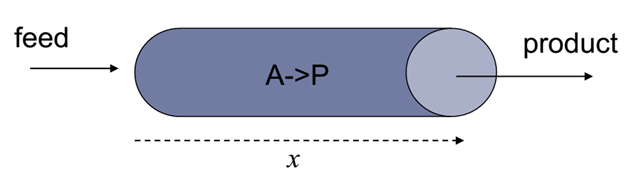
\includegraphics[width=.55\textwidth]{pfr}
 \end{center}
 \caption{A plug flow reactor.} 
 \label{fig:pfr}
\end{figure}

\noindent \textbf{Solution.} By following the modelling procedure discussed in Lecture 2,
we start by defining the necessary variables and their units:
\begin{align}
	0 \leq x \leq L; \quad &\textrm{$x$ - the spatial coordinate in axial direction; $L$ - length of the reactor [m]} \nonumber \\
	0 \leq t; \quad &\textrm{time [s]} \nonumber \\
	C_A(x, t); \quad &\textrm{concentration of reactant $A$ [kg m$^{-3}$]} \nonumber \\
	D; \quad &\textrm{diffusivity [m$^2$ s$^{-1}$]} \nonumber 	\\
	F;  \quad &\textrm{velocity of the fluid flow [m s$^{-1}$]} \nonumber 	\\
	r_A; \quad &\textrm{reaction rate [kg m$^{-3}$ s$^{-1}$]} \nonumber 
\end{align}

\noindent Now we can directly apply the general conservation equation (\ref{eq:conserv_pds_2}) for mass balance,
by substituting in the problem-specific variables. In particular:

\begin{center}
    \begin{tabular}{ l l | l l}
    \hline
    \multicolumn{2}{l|}{General equation (\ref{eq:conserv_pds_2})} &   \multicolumn{2}{l}{PFR example} \\
    \hline
    Symbol & Note & Symbol & Note \\
    \hline
    $\hat{\Phi}$ & volume-specific extensive variable & $C_A$ & concentration, i.e. volume-specific mass \\
    $v_x, v_y, v_z$ & velocity in three directions & $F$ & velocity in $x$ direction (1D problem) \\
    $\varphi$ & the potential corresponding to $\Phi$ & $C_A$ & concentration as potential in diffusion \\
    $\hat{q}$ & volume-specific generation rate of $\Phi$ & $r_A$ & reaction rate consuming $C_A$ \\
    \hline
    \end{tabular}
\end{center}

\noindent and thus the conservation equation becomes
\begin{equation} \label{eq:pfr_1}
	\frac{\partial C_A}{\partial t} = - F \frac{\partial C_A}{\partial x} + D \frac{\partial^2 C_A}{\partial x^2} - r_A
\end{equation}
\noindent Note that we can write a similar equation for the mass balance of 
chemical $P$ if the change of $P$ in the reactor is to be predicted.

We also need a constitutive equation for the reaction rate. Since this is known to be
a first-order reaction, we can relate $r_A$ to rate constant $k_A$ and concentration:
$r_A = k_A C_A$, where $k_A$ is usually written in the form of an
Arrhenius expression: $k_A = k_0 e^{-E/(RT)}$ and $k_0$ and $E$ can be experimentally determined;
see Lecture 3 for discussion of reaction kinetics.

Finally, we need to provide initial and boundary conditions so that eq. (\ref{eq:pfr_1}) can be
solved. We may use the following initial condition
\[ C_A(x, 0) = C_A^* \]
which means that at time $t=0$, the initial concentration of $A$ in the reactor 
is equal to $C_A^*$ which is uniform regardless of the spatial position $x$. Obviously,
the choice of initial condition must match the real situations.
Boundary condition is discussed next.

\end{exmp}


\subsection*{Boundary conditions}

\textbf{Number of boundary conditions.} The number of independent boundary conditions along a co-ordinate 
direction should be equal to the order of the corresponding partial derivative operator.

\begin{figure} [!h]
 \begin{center}
	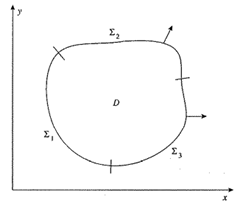
\includegraphics[width=.35\textwidth]{bdy}
 \end{center}
 \caption{Illustration of boundary conditions.}
 \label{fig:bdy}
\end{figure}

\textbf{Three types of boundary conditions.} Consider a general 2D surface\footnote{It's hard to visualise
a general 3D case, therefore we use 2D to illustrate the concept.} with two coordinates $x$ and $y$,
shown in Fig. \ref{fig:bdy}. The three types of boundary conditions are:
\begin{enumerate}
	\item \emph{The Dirichlet problem,} where the value of the differential variable
		is spcified on the boundary (denoted by $\Sigma_1$ in Fig. \ref{fig:bdy}):
		\[ \hat{\Phi} = f (x, y) \quad \textrm{on } \, \Sigma_1 \]
		\noindent where $f(x, y)$ is the function given by the modeller to specify the
		value of $\hat{\Phi}$ at spatial position $(x, y)$ on the boundary.
	\item \emph{The Neumann problem,} where the \emph{normal} derivative of the differential variable
		is spcified on the boundary (denoted by $\Sigma_2$ in Fig. \ref{fig:bdy}):
		\[ \frac{\partial \hat{\Phi}}{\partial n} = g(x, y) \quad \textrm{on } \, \Sigma_2 \]
		\noindent where $\partial \hat{\Phi} / \partial n$ refers to differentiation along the normal
		(perpendicular) to $\Sigma_2$ directed away from the interior of the balance volume $D$;
		$g(x, y)$ is the modeller-specified function.
	\item \emph{The Robbins problem,} also known as mixed condition, where we have
		\[ \alpha(x, y) \hat{\Phi} + \beta(x, y) \frac{\partial \hat{\Phi}}{\partial n} = \gamma (x, y) \quad \textrm{on } \, \Sigma_3 \]
		\noindent where $\alpha, \beta$ and $\gamma$ are modeller-specified functions.
\end{enumerate}

Returning to the plug flow reactor discussed in Example \ref{exmp:pfr}, it requires two boundary conditions along
the $x$ axis, because of the 2nd-order derivative term $\partial^2 C_A / \partial x^2$.
If we assume that (i) at the inlet ($x=0$), the concentration of $A$ is the same as that in the feed ($C_A^{(i)}$);
and (ii) the reactor is very long in the $x$ coordinate to enable full reaction, so that at the outlet ($x=L$)
the concentration does not change, we can write the boundary conditions as:
\[ C_A(0, t) = C_A^{(i)}; \quad \frac{\partial C_A}{\partial x} (L, t) = 0 \]


\begin{exmp}[A double-pipe heat exchanger]
\label{exmp:heat_exchg}
Consider a double pipe heated from outside by condensing saturated steam, shown in Fig. \ref{fig:heat_exchg}.
\textbf{Assumptions}: the overall mass of the liquid is constant; no diffusion takes place and heat conduction within the fluid
in the pipe is negligible; heat transfer coefficients, specific heats and densities are constant; time delays are negligible for fluid;
liquid is in plug flow. \textbf{Purpose of modelling}: To predict the change in the temperature in the exchanger over time and length.

\begin{figure} [!h]
 \begin{center}
	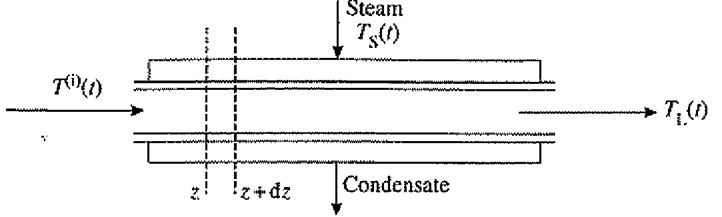
\includegraphics[width=.7\textwidth]{heat_exchg}
 \end{center}
 \caption{A double-pipe heat exchanger.} 
 \label{fig:heat_exchg}
\end{figure}

\noindent \textbf{Solution.} By following the modelling procedure discussed in Lecture 2,
we start by defining the necessary variables and their units:
\begin{align}
	0 \leq z \leq L; \quad &\textrm{$z$ - the spatial coordinate in axial direction; $L$ - length of the pipe [m]} \nonumber \\
	0 \leq t; \quad &\textrm{time [s]} \nonumber \\
	T_L(z, t); \quad &\textrm{temperature of fluid in the pipe [K]} \nonumber \\
	T_w(z, t); \quad &\textrm{temperature of the pipe wall [K]} \nonumber \\
	T_s(t); \quad &\textrm{temperature of the steam [K]} \nonumber 
\end{align}

\noindent where we have made some assumptions (it's always important to clearly state the assumptions made).
First, we decide that it's important to consider the pipe wall as a separate balance volume from
the fluid in the pipe. This is a typical choice, since the wall is made of a material (e.g. metal) that has very different
heat capacity from the fluid in the pipe, and it's reasonable to expect that heat transfer coefficient from steam to the wall
is very different from the heat transfer coefficient from wall to fluid. In addition, as the fluid is heated up as it
flows through the pipe, we expect temperature difference along the $z$ direction for the fluid ($T_L(z, t)$)
and for the wall ($T_w(z, t)$); however we assume the saturated steam's temperature does not change with
$z$; it may change with time though depending on the pressure of the steam supplied by the utility system, thus
denoted by $T_s(t)$.

Now we can directly apply the general conservation equation (\ref{eq:conserv_pds_2}) for energy balance,
by substituting in the problem-specific variables. Note that in eq. (\ref{eq:conserv_pds_2}), the extensive
variable $\hat{\Phi}$ is volume specific, while the relation between enthalpy and temperature, 
$\hat{H} = c_p T$, is mass specific. This means that when applying eq. (\ref{eq:conserv_pds_2}),
we need to ensure each term is mass specific. In particular:

\begin{center}
    \begin{tabular}{ l l | l l}
    \hline
    \multicolumn{2}{l|}{General equation (\ref{eq:conserv_pds_2}), now mass specific} &   \multicolumn{2}{l}{Heat exchanger example} \\
    \hline
    Symbol & Note & Symbol & Note \\
    \hline
    $\hat{\Phi}$ & specific extensive variable & $\hat{H}$ & specific enthalpy \\
    $v_x, v_y, v_z$ & velocity in three directions & $u$ & velocity in $z$ direction (1D problem) \\
    $\varphi$ & the potential corresponding to $\Phi$ & N.A. & heat conduction neglected  \\
    $\hat{q}$ & specific generation rate of $\Phi$ & $\hat{q}$ & specific heat transfer from wall to fluid \\
    \hline
    \end{tabular}
\end{center}

\noindent and thus the conservation equation becomes
\begin{equation} \label{eq:heat_exchg_1}
	\frac{\partial \hat{H}}{\partial t} = - u \frac{\partial \hat{H}}{\partial z} + \hat{q}
\end{equation}

\noindent Since it's temperature that is directly measured, we relate enthalpy to temperature $\hat{H} = c_{p,L} T$,
where $c_{p,L}$ [J kg$^{-1}$ K$^{-1}$] is the heat capacity of fluid in the pipe.
We also need a constitutive equation for the heat transfer term $\hat{q}$. 
Recall in Lecture 3 we expressed heat transfer as the product of \emph{overall} heat transfer coefficient
(here denoted by $h_L$ [W m$^{-2}$ K$^{-1}$]), heat transfer area $A$ and temeprature difference between
pipe wall and fluid ($T_w - T_L$), thus $q = h_L A (T_w - T_L)$.

However, in practice the information about heat transfer area is usually in the form of 
``internal pipe area per length of the pipe, $A_L$ [m$^{2}$/m]''. Imagine an infinitesimal segment of the pipe with
length of $dz$, as shown in Fig. \ref{fig:heat_exchg} between $z$ and $z + dz$, then the heat transfer area is
$A_L dz$ and thus the total heat transferred to this segment of fluid is $q = h_L A_L (T_w - T_L) dz$.
We need to further make this heat transfer mass-specific to be used in eq. \ref{eq:heat_exchg_1}), that is,
we divide $q$ by the mass of the fluid inside this infinitesimal segment:
\[ \hat{q} = \frac{q}{\rho A_f dz} = \frac{h_L A_L (T_w - T_L)}{\rho A_f} \]
where $A_f$ is the cross-section area of the fluid in the pipe. With these constitutive equations, 
eq. (\ref{eq:heat_exchg_1}) can be expanded to
\begin{equation} \label{eq:heat_exchg_2}
	c_{p,L} \frac{\partial T_L}{\partial t} = - u \, c_{p,L} \frac{\partial T_L}{\partial z} + \frac{h_L A_L (T_w - T_L)}{\rho A_f}
\end{equation}

Similarly we can develop an energy balance equation for the wall as balance volume (\textbf{verify this}):
\begin{equation} \label{eq:heat_exchg_3}
	M_w c_{p,w} \frac{\partial T_w}{\partial t} = - h_L A_L (T_w - T_L) + h_S A_s (T_s - T_w)
\end{equation}
\noindent where $h_S$ is the heat transfer coefficient from steam to wall, $A_S$ [m$^{2}$/m] the 
external pipe area per length of the pipe, $c_{p,w}$ the specific heat capacity of the wall,
and $M_w$ [kg/m] the mass of wall per length of the pipe.

Finally, we need to provide initial and boundary conditions. We may use the following initial conditions
\[ T_L(z, 0) = T^*, \quad  T_w(z, 0) = T^* \]
which means that at time $t=0$, the temperature of the fluid and wall is the same
and uniform regardless of the spatial position $z$. One could also set the initial condition as a function of $z$
if such information is available.
One boundary condition is needed for each of the two differential variables,
for only 1st order differentiations are involved along $z$ in modelling equations (\ref{eq:heat_exchg_2})(\ref{eq:heat_exchg_3}).
We can set $T_L(0, t) = T^{(i)}(t)$, i.e. the same as inlet fluid temperature,
but it's difficult to say anything about $T_w(0, t)$, the wall temperature at the inlet.
Instead we could set $\partial T_w(L, t) / \partial z = 0$, assuming the pipe is sufficiently
long and thus the wall temperature gradient along $z$ at the end of the pipe is negligible.

\end{exmp}


\section{Solution strategies}

Numerical solution of PDEs is a process which turns PDEs into ODEs or directly into algebraic equations 
which we know how to solve (numerically). Here we will briefly discuss two methods:
the finite difference method (FDM) that discretises a PDE fully into a set of algebraic equations,
and the method of lines (MoL) that discretise a PDE into a set of ODEs.
These methods are those most frequently used in process systems modelling; more advanced methods such as finite element method 
(FEM, often used in structural analysis) and finite volume method (FVM, often used in computational Fluid dynamics) exist.

\subsection*{Finite difference method}

Finite difference has been discussed in Lecture 5 when dealing with ODE solvers.
The same principle applies to PDEs. The idea is to replace the derivatives in the PDEs by finite difference,
discretising both spatial and temporal dimensions. 
Considering a uniform discretisation of a dimension $x$ (called meshing) from $a$ to $b$, 
shown in Fig. \ref{fig:fdm}, the $N+1$ discrete points (thus $N$ meshes) are represented as:

\[ x_i = a + i \cdot \delta x, \quad 0 < i < N \]
\[ \Delta x = (b - a)/N \]

\begin{figure} [!h]
 \begin{center}
	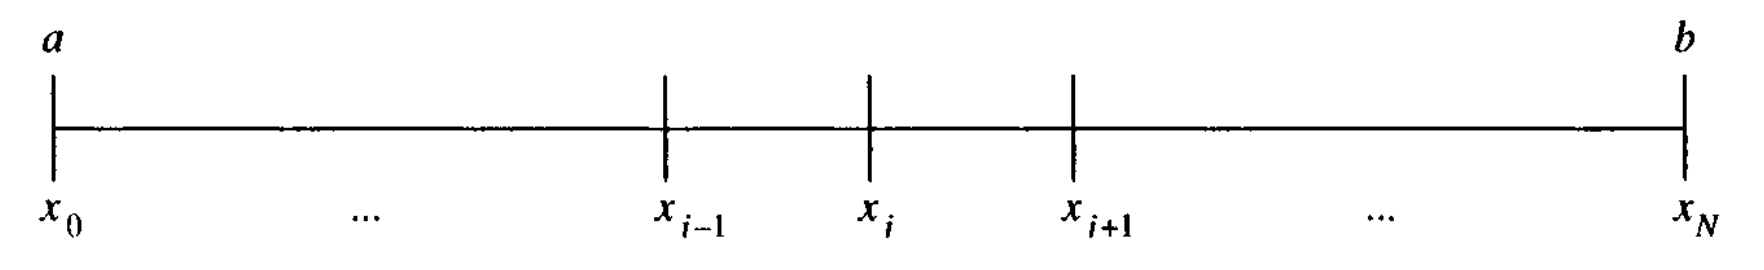
\includegraphics[width=.7\textwidth]{fdm}
 \end{center}
 \caption{Finite difference mesh.} 
 \label{fig:fdm}
\end{figure}

\noindent Then for any variable $u$ along this dimension, its derivatives can be approximated by
finite difference as:
\begin{align}
	\frac{d u(x_i)}{d x} &\approx \frac{u_{i+1} - u_i}{\Delta x}  \quad \textrm{(forward difference)} \nonumber \\
	\frac{d u(x_i)}{d x} &\approx \frac{u_i - u_{i-1}}{\Delta x}  \quad \textrm{(backward difference)} \nonumber 
\end{align}
\noindent and for 2nd order derivative, we can apply finite difference twice to get
\begin{align}
	\frac{d^2 u(x_i)}{d x^2} &\approx \frac{ \frac{u_{i+1} - u_i}{\Delta x} - \frac{u_i - u_{i-1}}{\Delta x}  }{ \Delta x} \nonumber \\
		&= \frac{u_{i+1} - 2 u_i + u_{i-1}}{\Delta x^2}  \nonumber
\end{align}
\noindent Higher-order derivatives can be approximated following the same principle.

\begin{exmp}[Finite difference method: an example]

Consider the following PDE
\[	\frac{\partial u}{\partial t} = \frac{\partial^2 u}{\partial x^2} \] 
defined on 1D coordinate $0 \leq x \leq 1$, with boundary conditions
\[ u(x=0, t) = 1, \quad u(x=1, t) = 0 \]
and initial conditions
\[ u(x, t=0) = \left\{ \begin{array}{ll}
	2x & \textrm{if} \; 0 \leq x \leq 0.5 \\
	2(1-x) & \textrm{if} \; 0.5 \leq x \leq 1\\
	\end{array} \right.
\]
We aim to solve the PDE from $t=0$ to $t=0.1$.

To solve the above PDE using the finite difference method,
we first define the discrete meshes upon which the solution will be calculated.
This is illlustrated in Fig. \ref{fig:fdm_mesh}, where the vertical axis represents
time $t$ and the horizontal axis spatial position $x$.

\begin{figure} [!h]
 \begin{center}
	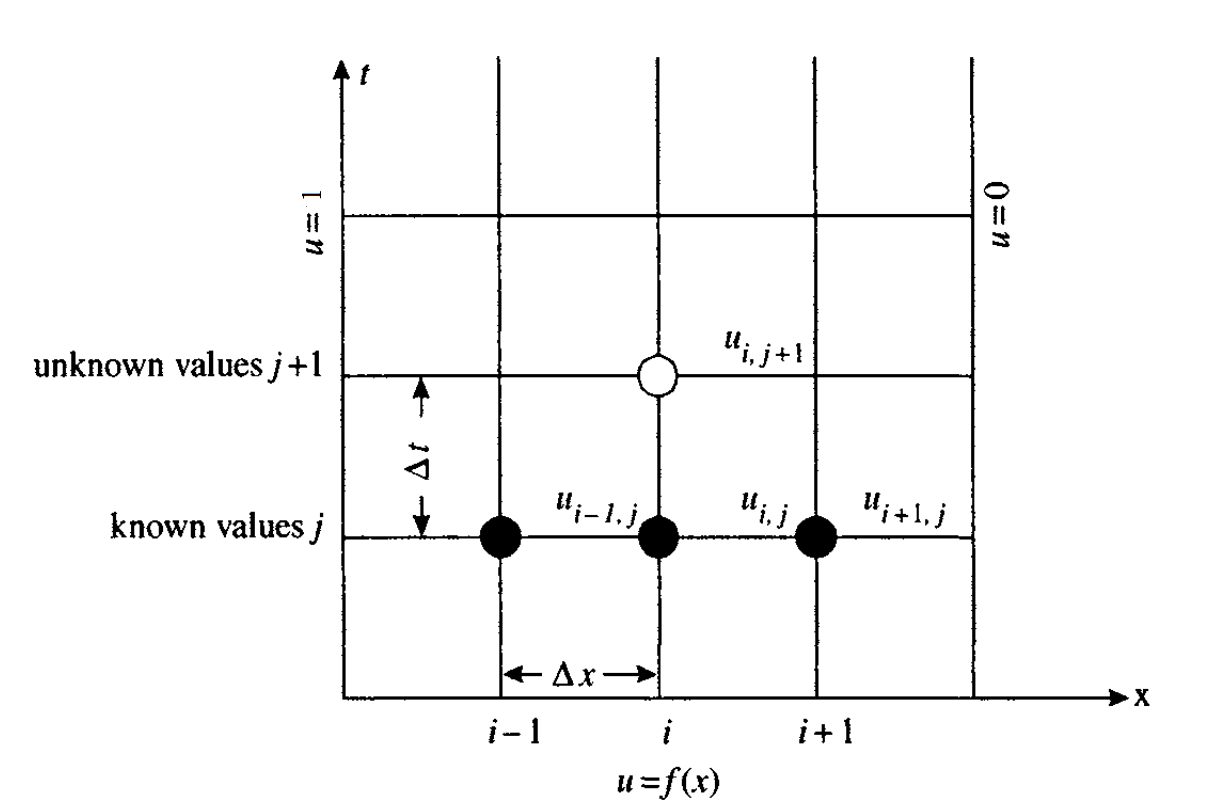
\includegraphics[width=.7\textwidth]{fdm_mesh}
 \end{center}
 \caption{Finite difference mesh with space $x$ and time $t$.} 
 \label{fig:fdm_mesh}
\end{figure}

The basic idea of finite difference is the discretise time and space into discrete points.
Here we discetise the $x$ axis into $N_x$ equal intervals ($i=0, 1, \ldots, N_x$), so the stepsize
$\Delta x = 1/N_x$ (note $0 \leq x \leq 1$ as given by the problem statement). Similarly we discretise
the $t$ axis into $N_t$ equal intervals ($j=0, 1, \ldots, N_t$) with a stepsize $\Delta t = 0.1/N_t$.
Now we want to compute the solutions at $u_{i,j}$.

As we have seen, there are different ways to approximate the derivatives
in finite difference (e.g. forward, backward, etc.). The following is one way to convert 
the PDE into a set of algebraic equations:
\[
	\frac{u_{i, j+1} - u_{i, j}}{\Delta t} = \frac{u_{i+1, j} - 2 u_{i, j} + u_{i-1, j}}{\Delta x^2}, \quad \textrm{for }
	i=0, 1, \ldots, N_x \textrm{ and }  j=0, 1, \ldots, N_t
\]
If it's not obvious how the above can be solved, let's re-arrange into
\begin{equation} \label{eq:fdm_exmp}
	u_{i, j+1} = u_{i, j} + \frac{\Delta t}{\Delta x^2} \left( u_{i+1, j} - 2 u_{i, j} + u_{i-1, j} \right)
\end{equation}
and notice the initial conditions mean $u_{i, 0}$ are known for any $i$,
and the boundary conditions translate into
\[
	u_{0,j} = 1, u_{N_x, j} = 0, \quad \textrm{for any } j
\]
Hence the computation starts from $j=0$ (i.e. $t=0$) where all $u_{i,0}$ are known. Then from
eq. (\ref{eq:fdm_exmp}) we can calculate $u_{i,1}$ (left-hand side) explicitly from
$u_{i,0}, u_{i+1,0}, u_{i-1,0}$ which are all known. Repeating this calculation for all meshes at $j=1$,
then move to the next time step $j=2$, and so on, until reaching $j=N_t$.

\textbf{The choice of $\Delta t$ and $\Delta x$} is an important but complicated matter.
The choice does not only affect accuracy but also stability of the solution. Here we consider three cases
as an example:
\begin{itemize}
	\item Case 1: $\Delta x=0.1, \Delta t=0.001$ (hence $N_x=10$ spatial steps and $N_t=100$ time steps), 
		and eq. (\ref{eq:fdm_exmp}) becomes
		\[ u_{i, j+1} = 0.1 \left( u_{i+1, j} + 8 u_{i, j} + u_{i-1, j} \right) \]
	\item Case 2: $\Delta x=0.1, \Delta t=0.005$ (hence $N_x=10$ spatial steps and $N_t=20$ time steps), 
		and eq. (\ref{eq:fdm_exmp}) becomes
		\[ u_{i, j+1} = 0.5 \left( u_{i+1, j} + u_{i-1, j} \right) \]
	\item Case 3: $\Delta x=0.1, \Delta t=0.01$ (hence $N_x=10$ spatial steps and $N_t=10$ time steps), 
		and eq. (\ref{eq:fdm_exmp}) becomes
		\[ u_{i, j+1} = u_{i+1, j} - u_{i, j} + u_{i-1, j} \]
\end{itemize}
You are encouraged to write a Matlab code to implement the three cases, and to compare the results.
For this particular example, the analytical solution exists. We compare the numerical solution with the analytical (true) solution
at a particular spatial position $x=0.3$ (i.e. $u_{3, j}$). The results are shown below:

 \begin{center}
	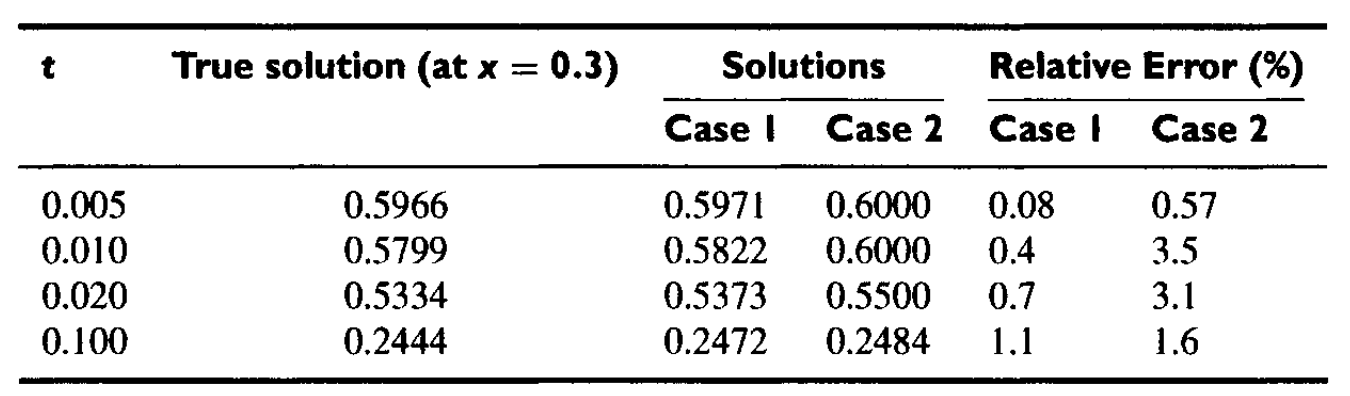
\includegraphics[width=.7\textwidth]{fdm_rlt}
 \end{center}

It appears that both case 1 and 2 provide reasonable accuracy, while case 1 is slightly more accurate
because of its smaller time steps. Case 3 is not illustrated because it produces totally wrong solution
with negative values of $u_{i,j}$ (use your Matlab code to verify this).

In general, the accuracy and stability depends on both $\Delta x$ and $\Delta t$, and for a given
$\Delta t$, decreasing $\Delta x$ will actually \textbf{de-stablise} the solution. 
Theoretical analysis of this topic is beyond the scope of this module.

\end{exmp}

\subsection*{Method of lines}

The idea of MoL is to discretise along only the spatial dimensions, but preserve time derivatives,
to convert a PDE to a set of ODEs. Then these ODEs can be solved by using the methods discussed in Lecture 4.
In a sense, MoL also falls within the family of finite difference, since the resultant ODEs will still be solved
based on the principle of finite difference. Nevertheless, many ODE solvers are available in many software packages,
so by using MoL the users do not have to worry about the time axis discretisation (which is automatically
dealt with by these mature solvers). We explain the idea of MoL through an example below.

\begin{exmp}[Method of lines: an example]

Consider the following PDE for $u(x, t)$
\[ \frac{\partial u}{\partial t} = \frac{\partial^2 u}{\partial x^2} - 0.5 \frac{\partial u}{\partial x} \]
defined on 1D space $0 \leq x \leq 1$ and time $t > 0$,
with the initial conditions:
\[ u(x, 0) = 0, \; 0 \leq x \leq 1 \]
and boundary conditions:
\[ u(0, t) = 1; \quad \frac{\partial u(1, t)}{\partial x} = 0 \]

Similar to the previous example, we discetise the $x$ axis into $N$ equal intervals ($i=0, 1, \ldots, N$), so the stepsize
$\Delta x = 1/N$ (note $0 \leq x \leq 1$ as given by the problem statement). We denote
the differential variable $u$ at each of these spatial points $u_i(t)$, and note $u_i(t)$ is located at the position
$x = i / N$. Also notice that $u_i(t)$ still depends on $t$, since in MoL we do not discretise the time axis.
Hence the derivatives at $u_i$ can be approximated as
\[ \frac{\partial u}{\partial x}\Big|_{u=u_i} \approx  \frac{u_{i+1} - u_i}{1/N} \]
\[ \frac{\partial^2 u}{\partial x^2}\Big|_{u=u_i} \approx  \frac{u_{i+1} - 2 u_i + u_{i-1}}{(1/N)^2} \]
\[ \frac{\partial u}{\partial t}\Big|_{u=u_i} = \frac{d u_i}{d t} \]
Therefore the resulting ODEs are:

\begin{equation} \label{eq:mol}
	\frac{d u_i}{d t} = \frac{u_{i+1} - 2 u_i + u_{i-1}}{(1/N)^2} - 0.5 \frac{u_{i+1} - u_i}{1/N},
	\quad i=1,\ldots,N
\end{equation}

The initial conditions in the PDE must be converted accordingly. They are
\[ u_i(0) = u(x = i / N, t=0) = 0, \quad i=1,\ldots,N \]

We also need to deal with the boundary conditions in the PDE. Note in eq. (\ref{eq:mol}),
when $i=1$, the right-hand side requires $u_2$, $u_1$ and $u_0$; $u_2$ and $u_1$ are part of the
ODEs to be solved for, but what about $u_0$? We can't simply extend eq. (\ref{eq:mol}) to 
solve for $u_0$ by using an index $i=0$, because if we do that, the right-hand side requires $u_{i-1}$
which is $u_{-1}$! What a vicious circle! We will run into a similar issue when $i=N$ and we need $u_{i+1}$
which is $u_{N+1}$.

The solution is at the boundary conditions, and it's simple. At the boundary $x=0$, 
$u_{x=0,t} = 1$, which means that $u_0(t) = 1$. Similarly at the boundary $x=1$,
we have $u_{N+1}(t) = u_N(t)$ (why?).

Putting everything together, the MoL converts the PDE into the following ODEs that can be solved
using the ODE solvers discussed before:
\begin{align}
	\frac{d u_i}{d t} &= \frac{u_{i+1} - 2 u_i + u_{i-1}}{(1/N)^2} - 0.5 \frac{u_{i+1} - u_i}{1/N},
	\quad i=1,\ldots,N \\
	u_i(0) &= 0, \quad i=1,\ldots,N \\
	u_0(t) &= 1, u_{N+1}(t) = u_N(t)
\end{align}

\end{exmp}

\begin{thebibliography}{2}
\vspace{-0.4cm}
\bibitem[{Hangos(2001)}]{Hangos2001}
	Hangos KM, Cameron IT, 2001. Process Modelling and Model Analysis, Academic Press: London.

\bibitem[{Smith(2004)}]{Smith2004}
	Smith JM, van Ness HC, Abbott MM, 2004. Introduction to Chemical Engineering Thermodynamics, 7th edition, McGraw-Hill.
\end{thebibliography}

\end{document}


